\documentclass[a4paper, 12pt]{article}
\usepackage[left=2cm, right=1cm, top=2cm, bottom=2cm]{geometry}
\usepackage[utf8]{inputenc}  % кодировка вводимого текста
\usepackage[english, russian]{babel}  % подключение словарей с переносами англ и рус яз
\usepackage{amssymb, latexsym, amsmath, mathtext, bm, gensymb, amssymb}  % пакеты для работы с мат символами
\usepackage{indentfirst}  %  каждый абзац с красной строки
\setlength{\parindent}{4ex}
\linespread{0.4} % межстрочный интервал
 
\usepackage{graphicx}
\graphicspath{ {./images/} }
\usepackage{float}
\usepackage{wrapfig}

\usepackage{bm}
\usepackage{enumitem}
\usepackage[T2A]{fontenc}

\usepackage{fancyhdr}

\usepackage[rightcaption]{sidecap}

\newcommand{\RNum}[1]{\uppercase\expandafter{\romannumeral #1\relax}}

\makeatletter
\AddEnumerateCounter{\asbuk}{\russian@alph}{щ}
\makeatother

% \pagestyle{fancy}
% \fancyhf{}
% \rhead{Саженов Константин Станиславович}
% \lhead{Группа М8О-108Б-19}
% \chead{Вариант 22}
% \rfoot{Page \thepage}
\setlength{\headheight}{28pt}
% \set
\addtocounter{MaxMatrixCols}{3}

\title{курсовая}

% variables
\newcommand{\E}{\begin{pmatrix}
    1 & 0 & 0 & 0 \\
    0 & 1 & 0 & 0 \\
    0 & 0 & 1 & 0 \\
    0 & 0 & 0 & 1
\end{pmatrix}} % E matrix

\newcommand{\A}{\begin{pmatrix}
    0 & 1 & 1 & 1 \\
    0 & 0 & 1 & 0 \\
    0 & 1 & 0 & 0 \\
    1 & 1 & 1 & 0
\end{pmatrix}} % A matrix

\newcommand{\Apowtwo}{\begin{pmatrix}
    1 & 1 & 1 & 0 \\
    0 & 1 & 0 & 0 \\
    0 & 0 & 1 & 0 \\
    0 & 1 & 1 & 1
\end{pmatrix}} % A ^ 2

\newcommand{\T}{\begin{pmatrix}
    1 & 1 & 1 & 1\\
    0 & 1 & 1 & 0\\
    0 & 1 & 1 & 0\\
    1 & 1 & 1 & 1
\end{pmatrix}} % T

\newcommand{\Smatrix}{\begin{pmatrix}
    1 & 0 & 0 & 1\\
    0 & 1 & 1 & 0\\
    0 & 1 & 1 & 0\\
    1 & 0 & 0 & 1
\end{pmatrix}} % S


\newcommand{\Sone}{\begin{pmatrix}
    0 & 0 & 0 & 0\\
    0 & 1 & 1 & 0\\
    0 & 1 & 1 & 0\\
    0 & 0 & 0 & 0
\end{pmatrix}} % S_1

\newcommand{\Omatrix}{\begin{pmatrix}
    0 & 0 & 0 & 0\\
    0 & 0 & 0 & 0\\
    0 & 0 & 0 & 0\\
    0 & 0 & 0 & 0
\end{pmatrix}} % S_2 == O

\newcommand{\K}{
    \begin{pmatrix}
        0 & 0 & 0 & 1\\
        0 & 0 & 1 & 0\\
        0 & 1 & 0 & 0\\
        1 & 0 & 0 & 0
    \end{pmatrix}
}

\newcommand{\thAmatrix}{
    \begin{pmatrix}
        0 & 0 & 0 & 0 & 1 & 1 & 0 \\
        1 & 0 & 1 & 0 & 1 & 1 & 0 \\
        1 & 1 & 0 & 1 & 1 & 0 & 0 \\
        0 & 0 & 1 & 0 & 1 & 1 & 1 \\
        1 & 1 & 0 & 0 & 0 & 1 & 0 \\
        0 & 0 & 1 & 0 & 1 & 0 & 0 \\
        1 & 1 & 0 & 1 & 1 & 0 & 0 
    \end{pmatrix}
}

\newcommand{\fAmatrix}{
    \begin{pmatrix}
        \infty & 2 & 7 & 8 & \infty & \infty & \infty \\
        12 & \infty & 4 & \infty & 6 & \infty & \infty \\
        \infty & 4 & \infty & 1 & 3 & 5 & 7 \\
        \infty & \infty & 1 & \infty & \infty & 3 & \infty \\
        \infty & \infty & 3 & \infty & \infty & \infty & 5 \\
        \infty & \infty & 5 & \infty & \infty & \infty & 2 \\
        2 & \infty & \infty & 3 & 4 & 6 & 7 
    \end{pmatrix}
}

\newcommand{\Cmatrix}{
    \begin{pmatrix}
        -1 & 1 & 0 & 0 & 0 & 0 & 1 & 0 & 0 & 0 & 0 & 0 & 0 \\
        0 & 0 & 1 & 0 & 0 & 0 & 1 & 0 & 0 & 0 & 1 & 1 & 0 \\
        0 & 0 & 0 & 1 & -1 & 0 & 0 & 0 & -1 & 0 & 1 & 0 & 0 \\
        0 & 0 & 0 & 0 & 0 & -1 & 0 & 0 & 1 & 0 & 0 & 1 & 0 \\
        0 & 1 & 0 & 0 & 0 & 0 & 1 & -1 & 0 & 0 & 0 & 1 & 0 \\
        0 & 0 & 0 & 1 & 0 & 0 & 0 & 0 & 0 & 1 & 1 & 0 & 0 \\
        0 & 0 & 0 & 0 & 0 & 0 & 1 & 0 & 0 & 0 & 0 & 1 & 1
    \end{pmatrix}
}

\newcommand{\Bmat}{
    \begin{pmatrix}
        -1 & -1 &  0 &  0 &  0 &  0 &  0 & -1 &  0 &  0 &  0 &  0 &  0 \\
         0 &  1 &  1 &  0 &  0 &  0 & -1 &  0 &  0 &  0 &  0 &  0 & -1 \\
         1 &  0 &  0 &  0 &  0 & -1 &  1 &  0 &  0 &  0 &  0 & -1 &  0 \\
         0 &  0 &  0 &  0 &  0 &  0 &  0 &  1 & -1 &  1 & -1 &  1 & -1 \\
         0 &  0 & -1 & -1 &  0 &  0 &  0 &  0 &  0 &  0 &  1 &  0 &  0 \\
         0 &  0 &  0 &  0 & -1 &  1 &  0 &  0 &  1 &  0 &  0 &  0 &  0 \\ 
         0 &  0 &  0 &  1 &  1 &  0 &  0 &  0 &  0 & -1 &  0 &  0 &  0 
    \end{pmatrix}
}

\newcommand{\Uvector}{
    \begin{pmatrix}
        U_1 \\ \vdots \\ U_{13}
    \end{pmatrix}
}

\newcommand{\Ivector}{
    \begin{pmatrix}
        I_1 \\ \vdots \\ I_{13}
    \end{pmatrix}
}

\begin{document}
\begin{titlepage}
    \begin{center}
    МИНИСТЕРСТВО ОБРАЗОВАНИЯ И НАУКИ РОССИЙСКОЙ ФЕДЕРАЦИИ
    
    Федеральное государственное бюджетное образовательное учреждение
    
    высшего образования
    
    
    «Московский Авиационный Институт
    
    (Национальный Исследовательский Университет)»
    
    ФАКУЛЬТЕТ ИНФОРМАЦИОННЫХ ТЕХНОЛОГИЙ И
    
    ПРИКЛАДНОЙ МАТЕМАТИКИ
    
    Кафедра вычислительной математики и программирования
    \vfill
    
    \textbf{КУРСОВАЯ РАБОТА}\\[5mm]
    по курсу «Дискретная математика»\\
    на тему «Теория графов»
    
    \end{center}
    \vfill
    
    \newlength{\ML}
    \settowidth{\ML}{«\underline{\hspace{0.7cm}}» \underline{\hspace{2cm}}}
    \hfill\begin{minipage}{0.4\textwidth}
    Студент: Саженов К. С.\\
    Группа М8О-108Б
    \end{minipage}%
    \bigskip
    
    \hfill\begin{minipage}{0.4\textwidth}
    Руководитель:\\
    Смерчинская С. О.
    \end{minipage}%
    \vfill
    
    \begin{center}
    Москва, 2020
    \end{center}
    \end{titlepage}
\section{Задание}
\subsection{Вариант 22}
\begin{enumerate}
    \item Определить для орграфа, заданной матрицей смежности:
    
    $ A = \begin{pmatrix}
        0 & 1 & 1 & 1 \\
        0 & 0 & 1 & 0 \\
        0 & 1 & 0 & 0 \\
        1 & 1 & 1 & 0
    \end{pmatrix} $
    \begin{enumerate}[label=\asbuk*)]
        \item матрицу односторонней связности
        \item матрицу сильной связности
        \item компоненты сильной связности
        \item матрицу контуров
    \end{enumerate}
    \item  Используя алгоритм Терри, определить замкнутый маршрут, проходящий ровно по два раза
    (по одному в каждом направлении) через каждое ребро графа.
    
    \includegraphics{2_task}
    \item  Используя алгоритм “фронта волны”, найти все минимальные пути из первой вершины в
    последнюю орграфа, заданного матрицей смежности.
    
    $ A = \thAmatrix $
    \item Используя алгоритм Форда, найти минимальные пути из первой вершины во все
    достижимые вершины в нагруженном графе, заданном матрицей длин дуг.

    $ A = \fAmatrix $
    \item Найти остовное дерево с минимальной суммой длин входящих в него ребер. % 2,8,1,7,6,4,3,2,9,8,4,5,1
    
    \includegraphics{5_graph}
    \newpage
    \item Пусть каждому ребру неориентированного графа соответствует некоторый элемент
    электрической цепи. Составить линейно независимые системы уравнений Кирхгофа для токов и
    напряжений. Пусть первому и пятому ребру соответствуют источники тока с ЭДС
    $E_1$ и $E_2$ (полярность выбирается произвольно), а остальные элементы являются сопротивлениями. Используя
    закон Ома, и, предполагая внутренние сопротивления источников тока равными нулю, получить
    систему уравнений для токов.
    
    \includegraphics{6_chain}

    \item Построить максимальный поток по транспортной сети. Начинать с окаймляющих цепей
    \begin{figure}[h]
        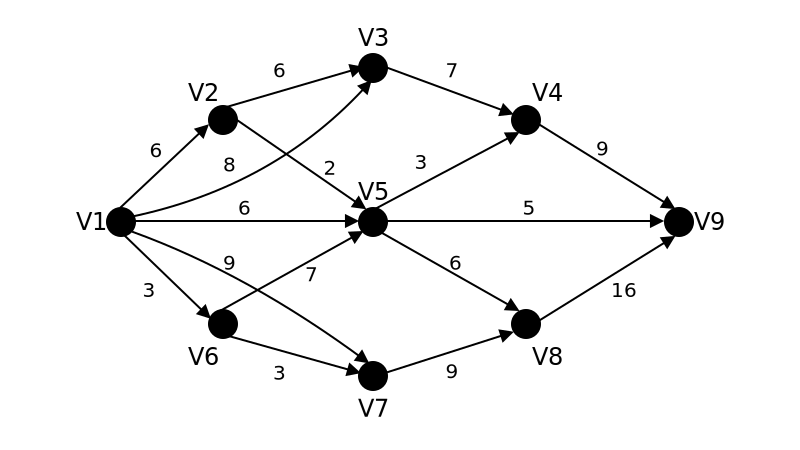
\includegraphics[width=360px]{7_flow}
    \end{figure}
    \item Раскраска вершин гиперграфа
\end{enumerate}
\newpage

\section{Задание \RNum{1}}
\begin{enumerate}[label=\asbuk*)]
    \item Найдем матрицу односторонней связности по формуле $ T = E \vee A \vee A^2 \vee A^3$:
    $$ E = \E $$
    $$
    A = \A
    $$
    $$
    A^2 = \A \ast \A = \Apowtwo
    $$
    $$
    A^3 = \Apowtwo \ast \A = \A
    $$

    $$
    T = \E \vee \A \vee \Apowtwo \vee \A = \T
    $$
    $ T = \T$ - матрица односторонней связности
    \item Найдем матрицу сильной связности по формуле $ S = T \& T^T$:
    $$ \bar{S} = \T \& 
    \begin{pmatrix}
        1 & 0 & 0 & 1\\
        1 & 1 & 1 & 1\\
        1 & 1 & 1 & 1\\
        1 & 0 & 0 & 1
    \end{pmatrix} = \Smatrix
    $$
    $ \bar{S} = \Smatrix$ - матрица сильной связности
    
    \item Компоненты сильной связности:
    $$ \bar{S} = \Smatrix $$
    $$ \{v_1, v_4\} \text{ -- первая компонента сильной связности} $$
    $$ \bar{S}_1  = \Sone $$
    $$ \{v_2, v_3\} \text{ -- вторая компонента сильной связности}$$
    $$ \bar{S}_2 = \Omatrix = O $$
    $$ \bar{S}_2 = O \Rightarrow \bar{S}_2 - \text{нулевая матрица, значит компонент больше нет} $$
    \item Матрица контуров $ K = \bar{S} \& A $
    $$ K = \Smatrix \& \A = \K \Rightarrow \text{дуги:} \left<v_1,v_4\right>, \left<v_4,v_1\right>, \left<v_2,v_3\right>, \left<v_3,v_2\right>$$
\end{enumerate}

\section{Задание \RNum{2}} 
$$ 1 \rightarrow 4 \rightarrow 3 \rightarrow 5 \rightarrow 6 \rightarrow 2 \rightarrow 3 \rightarrow 2 \rightarrow 6 \rightarrow 1 \rightarrow 6 \rightarrow 5 \rightarrow 3 \rightarrow 4 \rightarrow 1$$

\section{Задание \RNum{3}}

\begin{figure}[h]
    \includegraphics{3_graph}
\end{figure}

$ \left. 
\begin{aligned}
    v_1 &\in W_0 \\ 
    \Gamma _{W_1}(v1) &= \{v_5, v_6\} \\
    \Gamma _{W_2}(v1) &= \{v_2, v_3\} \\
    \Gamma _{W_3}(v1) &= \{v_4\} \\
    \Gamma _{W_4}(v1) &= \{v_7\}
\end{aligned}
\right\} \Rightarrow $ длина кратчайшего пути равна $4$.

\noindent Найдем кратчайший путь:
\begin{enumerate} %[label=\arabic*)]
    \item $v_7$
    \item $ \Gamma_{v_7}^{-1} \cap W_3(v_1) = \{v_4\} \cap \{v_4\} = \{v_4\}$
    \item $ \Gamma_{v_4}^{-1} \cap W_2(v_1) = \{v_3, v_7\} \cap \{v_2, v_3\} = \{v_3\}$
    \item $ \Gamma_{v_3}^{-1} \cap W_1(v_1) = \{v_2, v_4, v_6\} \cap \{v_5, v_6\} = \{v_6\}$
    \item $ \Gamma_{v_6}^{-1} \cap W_0(v_1) = \{v_1, v_2, v_4, v_5\} \cap \{v_1\} = \{v_1\}$
\end{enumerate}
$ v_1 \rightarrow v_6 \rightarrow v_3 \rightarrow v_4 \rightarrow v_7$ - единственный кратчайший путь. Длина кратчайшего пути 4

\section{Задание \RNum{4}} 

$$\begin{tabular}{ c| c| c |c| c| c| c| c|c| c |c |c |c|c| c| }
    & $v_1$ & $v_2$ & $v_3$ & $v_4$ & $v_5$ & $v_6$ & $v_7$ & $\lambda_i^{(0)}$ & $\lambda_i^{(1)}$ & $\lambda_i^{(2)}$ & $\lambda_i^{(3)}$ & $\lambda_i^{(4)}$ & $\lambda_i^{(5)}$ & $\lambda_i^{(6)}$\\ \hline
    $v_1$ & $\infty$ & 2 & 7 & 8 & $\infty$ & $\infty$ & $\infty$ & 0 & 0 & 0 & 0 & 0 & 0 & 0 \\ \hline
    $v_2$ & 12 & $\infty$ & 4 & $\infty$ & 6 & $\infty$ & $\infty$ & $\infty$ & 2 & 2 & 2 & 2 & 2 & 2\\ \hline
    $v_3$ & $\infty$ & 4 & $\infty$ & 1 & 3 & 5 & 7 & $\infty$ & 7 & 6 & 6 & 6 & 6 & 6 \\ \hline
    $v_4$ & $\infty$ & $\infty$ & 1 & $\infty$ & $\infty$ & 3 & $\infty$ & $\infty$ & 8 & 8 & 7 & 7 & 7 & 7\\ \hline
    $v_5$ & $\infty$ & $\infty$ & 3 & $\infty$ & $\infty$ & $\infty$ & 5 & $\infty$ & $\infty$ & 8 & 8 & 8 & 8 & 8\\ \hline
    $v_6$ & $\infty$ & $\infty$ & 5 & $\infty$ & $\infty$ & $\infty$ & 2 & $\infty$ & $\infty$ & 11 & 11 & 10 & 10 & 10\\ \hline
    $v_7$ & 2 & $\infty$ & $\infty$ & 3 & 4 & 6 & 7  & $\infty$ & $\infty$ & 14 & 13 & 13 & 12 & 12 \\ \hline
    \end{tabular}$$ 
    \begin{enumerate}
        \setcounter{enumi}{1}
        \item Длины минимальных путей из вершины $v_1$ во все остальные вершины определены в последнем столбце таблицы.
        \item Найдем вершины, входящие в минимальные пути из $v_1$ во все остальные вершины графа:
        \begin{enumerate}[label*=\arabic*.]
            \item Минимальный путь из $v_1$ в $v_2$: $v_1 \rightarrow v_2$, его длина -- 2
            $$ \lambda_1^{(0)} + c_{12} = 0 + 2 = \lambda_2^{(1)} $$
            \item Минимальный путь из $v_1$ в $v_3$: $v_1 \rightarrow v_2 \rightarrow v_3$, его длина -- 6
            \begin{align*}
                \lambda_1^{(0)} + c_{13} &= 0 + 7 = 7 = \lambda_3^{(1)} \\
                \lambda_2^{(1)} + c_{23} &= 2 + 4 = 6 = \lambda_3^{(2)}
            \end{align*}
            \item Минимальный путь из $v_1$ в $v_4$: $v_1 \rightarrow v_2 \rightarrow v_3 \rightarrow v_4 $, его длина -- 7
            \begin{align*}
                \lambda_3^{(2)} + c_{34} &= 6 + 1 = 7 = \lambda_4^{(3)} \\
                \lambda_2^{(1)} + c_{23} &= 2 + 4 = 6 = \lambda_3^{(2)} \\
                \lambda_1^{(0)} + c_{12} &= 0 + 2 = 2 = \lambda_2^{(1)}
            \end{align*}
            \item Минимальный путь из $v_1$ в $v_5$: $v_1 \rightarrow v_2 \rightarrow v_5$, его длина -- 8
            \begin{align*}
                \lambda_2^{(1)} + c_{25} &= 2 + 6 = 6 = \lambda_5^{(2)} \\
                \lambda_1^{(0)} + c_{12} &= 0 + 2 = 2 = \lambda_2^{(1)}
            \end{align*}
            \item Минимальный путь из $v_1$ в $v_6$: $v_1 \rightarrow v_2 \rightarrow v_3 \rightarrow v_4 \rightarrow v_6$, его длина -- 10
            \begin{align*}
                \lambda_4^{(3)} + c_{46} &= 7 + 3 = 10 = \lambda_6^{(4)} \\
                \lambda_3^{(2)} + c_{34} &= 6 + 1 = 7 = \lambda_4^{(3)} \\
                \lambda_2^{(1)} + c_{23} &= 2 + 4 = 6 = \lambda_3^{(2)} \\
                \lambda_1^{(0)} + c_{12} &= 0 + 2 = 2 = \lambda_2^{(1)}
            \end{align*}
            \item Минимальный путь из $v_1$ в $v_7$: $v_1 \rightarrow v_2 \rightarrow v_3 \rightarrow v_4 \rightarrow v_6 \rightarrow v_7$, его длина -- 12
            \begin{align*}
                \lambda_6^{(3)} + c_{67} &= 10 + 2 = 12 = \lambda_7^{(5)} \\
                \lambda_4^{(3)} + c_{46} &= 7 + 3 = 10 = \lambda_6^{(4)} \\
                \lambda_3^{(2)} + c_{34} &= 6 + 1 = 7 = \lambda_4^{(3)} \\
                \lambda_2^{(1)} + c_{23} &= 2 + 4 = 6 = \lambda_3^{(2)} \\
                \lambda_1^{(0)} + c_{12} &= 0 + 2 = 2 = \lambda_2^{(1)}
            \end{align*}
        \end{enumerate}
    \end{enumerate}

\section{Задание \RNum{5}}
\begin{enumerate}
    \item Добавляем дуги с весом $1$: $x_3,x_{13}$. Циклов нет
    \item Добавляем дуги с весом $2$: $x_1, x_8$. Циклов нет
    \item Добавляем дуги с весом $3$: $x_7$. Циклов нет
    \item Добавляем дуги с весом $4$: $x_6, x_{11}$. Циклов нет
    \item Добавялем дуги с весом $5$: $x_{16}, x_{12}, x_{15}$. Если добавить ещё $x_{17}$, то будет цикл
    \item Добавляем дуги с весом $6$: $x_5$. Циклов нет. Минимальное остовное дерево построено
\end{enumerate}
$$ L(D) = 1\cdot2 + 2 \cdot 2 + 3 \cdot 1 + 4 \cdot 2 + 5 \cdot 3 + 6 = 38$$
38 - минимальный вес остовного дерева

\includegraphics{5_tree}

\section{Задание \RNum{6}}
\begin{enumerate}
    \item Зададим произвольную ориентацию:
    \begin{figure}[h]
        \includegraphics{6_orgraph}
    \end{figure}
    \item Построим произвольное остовное дерево:
    \begin{figure}[h]
        \includegraphics{6_tree}
    \end{figure}
    \begin{enumerate}[label*=\arabic*.]
        \item $ D_1 = (U_1, \emptyset) $
        \item $ D_2 = (\{U_{ 1}, U_{ 2}\}, \{U_{ 1}, U_{ 2}\})$
        \item $ D_3 = (\{U_{ 1}, U_{ 2}, U_{ 3}\}, \{U_{ 1}, U_{ 2}\}, \{U_{ 2}, U_{ 3}\})$
        % \newpage
        \item $ D_4 = D_3 + \{U_{ 4}\} + \{U_{ 3}, U_{ 4}\} $
        \item $ D_5 = D_4 + \{U_{ 5}\} + \{U_{ 5}, U_{ 4}\} $
        \item $ D_6 = D_5 + \{U_{ 7}\} + \{U_{ 5}, U_{ 7}\} $
        \item $ D_7 = D_6 + \{U_{ 6}\} + \{U_{ 6}, U_{ 4}\} $
    \end{enumerate}
    \item Найдем базис циклов:
    \begin{enumerate}[label*=\arabic*.]
        \item 
        $(D + q_1) : \mu_1 : U_1 - U_2 - U_3 - U_1 \Rightarrow C(\mu_1) = 
            \begin{pmatrix}
            -1 & 1 & 0 & 0 & 0 & 0 & 1 & 0 & 0 & 0 & 0 & 0 & 0
            \end{pmatrix} 
        $
        \item 
        $(D + q_3) : \mu_2 : U_2 - U_3 - U_4 - U_5 - U_2 \Rightarrow C(\mu_2) = 
            \begin{pmatrix}
            0 & 0 & 1 & 0 & 0 & 0 & 1 & 0 & 0 & 0 & 1 & 1 & 0
            \end{pmatrix} 
        $
        \item 
        $(D + q_5) : \mu_3 : U_4 - U_5 - U_7 - U_6 - U_4 \Rightarrow C(\mu_3) = 
            \begin{pmatrix}
            0 & 0 & 0 & 1 & -1 & 0 & 0 & 0 & -1 & 0 & 1 & 0 & 0
            \end{pmatrix} 
        $
        \item 
        $(D + q_6) : \mu_4 : U_3 - U_4 - U_6 - U_3 \Rightarrow C(\mu_4) = 
            \begin{pmatrix}
            0 & 0 & 0 & 0 & 0 & -1 & 0 & 0 & 1 & 0 & 0 & 1 & 0
            \end{pmatrix} 
        $
        \item 
        $(D + q_8) : \mu_5 : U_1 - U_2 - U_3 - U_4 - U_1 \Rightarrow C(\mu_5) = 
            \begin{pmatrix}
            0 & 1 & 0 & 0 & 0 & 0 & 1 & -1 & 0 & 0 & 0 & 1 & 0
            \end{pmatrix} 
        $
        \item 
        $(D + q_{10}) : \mu_6 : U_4 - U_5 - U_7 - U_4 \Rightarrow C(\mu_6) = 
            \begin{pmatrix}
            0 & 0 & 0 & 1 & 0 & 0 & 0 & 0 & 0 & 1 & 1 & 0 & 0
            \end{pmatrix} 
        $
        \item 
        $(D + q_{13}) : \mu_7 : U_2 - U_3 - U_4 - U_2 \Rightarrow C(\mu_7) = 
            \begin{pmatrix}
            0 & 0 & 0 & 0 & 0 & 0 & 1 & 0 & 0 & 0 & 0 & 1 & 1
            \end{pmatrix} 
        $
        
    \end{enumerate}
    \item Цикломатическая матрица графа имеет вид:
    $$ C = \Cmatrix $$
    \item Выпишем закон Кирхгофа для напряжений: \\
    $ \Cmatrix \Uvector = 0 \Longleftrightarrow \left\{\begin{array}{lcl}
        -U_1 + U_2 + U_7 = 0\\
        U_3 + U_7 + U_{11} + U_{12} = 0 \\
        U_4 - U_5 - U_9 + U_{11} = 0 \\
        -U_6 + U_9 + U_{12} = 0 \\
        U_7 - U_8 + U_{12} = 0 \\
        U_4 + U_{10} + U_{11} = 0 \\
        U_7 + U_{12} + U_{13} = 0
    \end{array} \right. \\ \Longrightarrow 
    \left\{ \begin{array}{lcl}
        U_1 = U_2 + U_7 \\ 
        U_3 = -U_7 - U_{11} - U_{12} \\ 
        U_5 = U_4 - U_9 + U_{11}\\ 
        U_6 = U_9 + U_{12}\\ 
        U_8 = U_7 + U_{12}\\
        U_{10} = -U_4 - U_{11}\\
        U_{13} = -U_7 - U_{12}
    \end{array}\right.$
    \item Найдем матрицу инцидентности $B$ орграфа:
    $$\begin{tabular}{ c| c| c |c| c| c| c| c|c| c |c |c |c |c |}
        & $q_1$ & $q_2$ & $q_3$ & $q_4$ & $q_5$ & $q_6$ & $q_7$ & $q_8$ & $q_9$ & $q_{10}$ & $q_{11}$ & $q_{12}$ & $q_{13}$\\ \hline
        $U_1$ & -1 & -1 &  0 &  0 &  0 &  0 &  0 & -1 &  0 &  0 &  0 &  0 &  0 \\ \hline
        $U_2$ &  0 &  1 &  1 &  0 &  0 &  0 & -1 &  0 &  0 &  0 &  0 &  0 & -1 \\ \hline
        $U_3$ &  1 &  0 &  0 &  0 &  0 & -1 &  1 &  0 &  0 &  0 &  0 & -1 &  0 \\ \hline
        $U_4$ &  0 &  0 &  0 &  0 &  0 &  0 &  0 &  1 & -1 &  1 & -1 &  1 & -1 \\ \hline
        $U_5$ &  0 &  0 & -1 & -1 &  0 &  0 &  0 &  0 &  0 &  0 &  1 &  0 &  0 \\ \hline
        $U_6$ &  0 &  0 &  0 &  0 & -1 &  1 &  0 &  0 &  1 &  0 &  0 &  0 &  0 \\ \hline
        $U_7$ &  0 &  0 &  0 &  1 &  1 &  0 &  0 &  0 &  0 & -1 &  0 &  0 &  0 \\ \hline
        \end{tabular}
        $$
        $$ B = \Bmat $$
    % \newpage
    \item Выпишем уравнения Кирхгофа для токов:
    $$ \Bmat \cdot \Ivector = 0 \Rightarrow $$
    \begin{align}\left\{ \begin{array}{lcr}
        I_1 + I_2 + I_8 = 0 \\
        I_2 + I_3 - I_7 + I_{13} = 0 \\
        I_1 - I_6 + I_7 - I_{12} = 0 \\
        I_{11} - I_3 - I_4 = 0 \\
        I_{7} - I_6 + I_9 = 0 \\
        I_{5} + I_6 - I_{10} = 0 
    \end{array} \right. \end{align}
    \item Подставим закон Ома:
    \begin{align}
        \left\{ \begin{array}{lcr}
            E_1 = I_2 R_2 + I_7 R_7 \\
            E_2 = I_4 R_4 - I_9 R_9 + I_{11} R_{11} \\
            I_3 R_3 + I_7 R_7 + I_{11} R_{11} + I_{12} R_{12} = 0 \\
            I_6 R_6 - I_9 R_9 - I_{12} R_{12} = 0 \\
            I_8 R_8 - I_7 R_7 - I_{12} R_{12} = 0 \\
            I_{10} R_{10} + I_4 R_4 + I_{11} R_{11} = 0 \\
            I_{13} R_{13} I_7 R_7 + I_{12} R_{12} = 0
        \end{array}\right.
    \end{align}
    \item Совместная система состоит из систем (1) и (2). 13 уравнений и 13 неизвестных -- 
    токи $ I_1 \dots I_{13} ;$ ЭДС $ E_1, E_2$ Сопротивления $R_2 ; R_3 ; R_4 ; R_5 ; R_6 ; R_7 ; R_8 ; R_9 ; R_{10} ; R_{11} ; R_{12} ; R_{13}$ - известны
\end{enumerate}

% \newpage
\section{Задание \RNum{7}} 
\paragraph{Текст задания} Построить максимальный поток по транспортной сети. Начинать с окаймляющих цепей
\begin{figure}[h]
    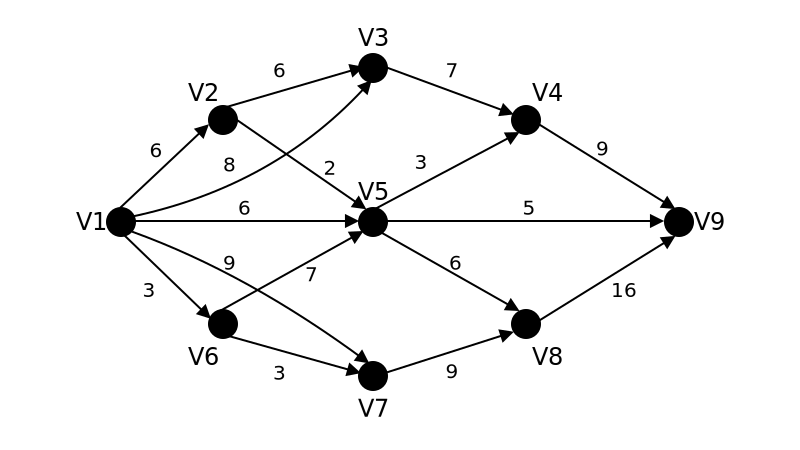
\includegraphics[width=360px]{7_flow}
\end{figure}
\begin{enumerate}
    \item Построение полного потока:
    \begin{align*}
        v_1 \rightarrow v_2 \rightarrow v_3 \rightarrow v_4 \rightarrow v_5\\
        \min\{6, 6, 7, 9\} = 6
    \end{align*}
    \begin{align*}
        v_1 \rightarrow v_8 \rightarrow v_7 \rightarrow v_6 \rightarrow v_5 \\
        \min\{3, 3, 9, 16\} = 3 
    \end{align*}
    \begin{align*}
        v_1 \rightarrow v_9 \rightarrow v_5\\
        \min\{6, 5\} = 5 
    \end{align*}
    \begin{align*}
        v_1 \rightarrow v_3 \rightarrow v_4 \rightarrow v_5\\
        \min\{8, 7-6, 9-6\} = 1
    \end{align*}
    \begin{align*}
        v_1 \rightarrow v_7 \rightarrow v_6 \rightarrow v_5\\
        \min\{9, 9-3, 16-3\} = 6
    \end{align*}
    \begin{align*}
        v_1 \rightarrow v_9 \rightarrow v_4 \rightarrow v_5\\
        \min\{6-5, 3, 9-7\} = 1
    \end{align*}
    $$ \Phi _{полн.} = 1 +6 +1 + 3+6 + 5 = 22$$
    \item Построение максимального потока:
    \begin{enumerate}
        \item $ v_1 \rightarrow v_3 \rightarrow v_2 \rightarrow v_9 \rightarrow v_4 \rightarrow v_5 $
        $$ \Delta_1 = \min\{8-1, 6, 2, 2-1, 9-8\} = 1$$ 
        \item $ v_1 \rightarrow v_3 \rightarrow v_2 \rightarrow v_9 \rightarrow v_6 \rightarrow v_5 $
        $$ \Delta_2 = \min\{8-2, 5, 2-1, 4, 16-9\} = 1$$ 
        \item $ v_1 \rightarrow v_7 \rightarrow v_8 \rightarrow v_9 \rightarrow v_6 \rightarrow v_5 $
        $$ \Delta_3 = \min\{9-6, 3, 7, 6-1, 16-9\} = 3$$ 
    \end{enumerate}
    $$ \Phi_{макс.} = 9 + 5+13=27$$
\end{enumerate}
Величина $|f|$ равна $27$.

\section{Задание \RNum{8}}
\subsection{Теоретические сведения}
Гиперграф($H$) -- обобщение простого графа. В гиперграфе ребрами могут быть любые подмножества множества вершин графа. 

Пусть $V$ – конечное непустое множество, $E$ – некоторое семейство непустых различных
подмножеств множества $V$ . Пара $(V, E)$ называется гиперграфом с множеством \emph{вершин} $V$
и множеством \emph{ребер}(\emph{гиперребер}) $E$.

Если вершина $ v \in V$ принадлежит ребру $e \in E$, то будем называть вершину и ребро \emph{инцилентными} друг другу.
Число $|E(v)|$ называется \emph{степенью вершины} $v$, а $|e|$ -- \emph{степенью ребра} $e$. Вершина гиперграфа, не 
инцидентная никакому ребру, называется \emph{изолированной}.

Для любого гиперграфа можно определить граф инциденций -- \emph{двудольный} граф с множеством вершин 
$ V \cup E $ и множеством ребер $ \{(v, e): (v, e) \in V \times E, v\in e\} $.

Для гиперграфов также существует понятие вершинной раскраски. Раскраску вершин гиперграфа будем называть \emph{правильной}, 
если две вершины $v_i, v_j $, принадлежащие одному ребру $ e_k $ имеют разные цвета $v_i, v_j \in e_k, i \neq j : Color(v_i) \neq Color(v_j)$.

\emph{Хроматическое число} $ \chi(H) $ -- наименьшее число цветов, достаточное для правильной раскраски гиперграфа $H$.

\emph{Двудольный граф} -- граф, множество вершин которого можно разбить на две части таким образом, 
что каждое ребро графа соединяет какую-то вершину из одной части с какой-то вершиной другой части, то есть не существует рёбер между вершинами одной и той же части.

\emph{Клика} размера $n$ (обозначается $K_n$) -- полный подграф размера $n$ обычного графа 

\subsection{Описание алгоритма}

\begin{enumerate}
    \item Гиперграф задается с помощью матрицы инцидентности, где любое число не равное 0 - означает принадлежность вершины к ребру,
    а 0 - отсутствие вершины в данном гиперребре.
    \item Для начала требуется преобразовать матрицу смежности в список смежности, для этого:\begin{enumerate}
        \item Преобразовываем матрицу инцидентности в матрицу смежности с кликами, вместо гиперребер
        \item Преобразуем матрицу смежности в матрицу инцидентности с обычными ребрами
        \item Преобразуем матрицу инцидентности в список смежности вершин
    \end{enumerate}
    \item Раскрашиваем граф: \begin{enumerate}
        \item Окрашиваем первую вершину в цвет $c_0$
        \item Выбрать цвет окраски $c_0$
        \item Пока не покрашены все вершины, повторять пункты i, ii: \begin{enumerate}
            \item Окрасить в выбранный цвет каждую вершину, которая не смежна с другой, уже окрашенной в этот цвет.
            \item Выбрать цвет $c_j = c_{i+1}$, $c_i$ - предыдущий цвет
        \end{enumerate}
    \end{enumerate}
\end{enumerate}

\subsection{Блок-схема алгоритма}

% \begin{figure}[h]
    \includegraphics{8_block}
    % \caption{Блок-схема}
% \end{figure}

Программа написана на языке C++ с использованием фреймворка Qt версии 5.14 и набора утилит GraphViz

\subsection{Оценка сложности алгоритма}
В данном алгоритме происходят преобразования матриц/списков друг в друга. 
Данные операции выполняются за $O(n^2)$ времени. Также при основном алгоритме происходит перебор каждой вершины графа за $O(n)$ и, 
затем для каждой вершины требуется найти минимальный цвет, что в худшем случае может иметь сложность $O(n^2)$. 
Следовательно, общее время работы алгоритма $O(n^3)$

\subsection{Тестовые примеры. Скриншоты программ}

\textbf{Пример 1.} Вводится частный случай гиперграфа с 6 вершинами и 3 ребрами. Граф представлен на Рис.:

% \begin{figure}[h]
%     % \centering
%     \begin{center}
        \includegraphics[scale=0.5]{8_true_graph}
%     \end{center}
    % \caption{Частный случай гиперграфа}
% \end{figure}


% \begin{figure}[h]
%     % \centering
%     \begin{center}
        \includegraphics[width=200px]{8_program}
%     \end{center}
%     \caption{Представление гиперграфа в виде двудольного, вид программы и матрица инцидентности}
% \end{figure}


\textbf{Пример 2.} Дан гиперграф:

% \begin{figure}[h]
%     % \centering
%     \begin{center}
        \includegraphics[width=100px]{8_2_true_graph.png}
%     \end{center}
%     \caption{Гиперграф}
% \end{figure}

% \begin{figure}[h]
%     % \centering
%     \begin{center}
        \includegraphics[width=200px]{8_2_program}
%     \end{center}
%     \caption{Представление гиперграфа в виде двудольного, вид программы и матрица инцидентности}
% \end{figure}

\section{Примеры прикладных задач}
Для частного случая гиперграфа можно рассматривать задачу кадендарного/временного планирования каких-либо операций, например
операций-преобразований в компьютере. Каждой операции следует сопоставить вершину графа, причем любые две вершины будут соединены ребром только тогда,
когда соответствующие им операции-преобразования не могут быть осуществлены одновременно. 
Требуется составить такой план операций, который связан с наименьшими временными затратами.
Задача эквивалентна задаче о раскраске вершин графа с использованием наименьшего числа цветов.

Для гиперграфа можно определить задачу распределения ключей безопасности для шифрования данных в сети Tor.
Каждой подсети сети Tor будет соответствовать гиперребро, в то время как каждому узлу в каждой подсети(подсети могут пересекаться)
будет соответствовать вершина гиперграфа. Тогда задача, с точки зрения безопасности данных, состоит в следующем:
каким образом разбить данные на $K$ независимых частей и эти части разбить на $K_i$ зависимых частей, где $i$ - номер подсети в сети Tor,
чтобы каждый узел в каждой подсети имел только ту часть зашифрованных данных, которая нужна для полноценной безопасной передачи данных.
Причем разбить данные следует "наилучшим" способом, то есть производя наименьшее количество итераций шифровки-дешифровки.
Эта задача эквивалентна задаче о нахождении минимальной раскраски в гиперграфе.

\newpage
\begin{thebibliography}{3}
    \addcontentsline{toc}{section}{\bibname}
    \bibitem{Nicos}Никос Кристофидес. Теория графов: алгоритмический подход. М.: Мир, 1978. - 423 стр.
    \bibitem{Emelnikov}Емеличев В.А. Лекции по теории графов. М.: Наука, 1990. - 384 стр.
    \bibitem{mipt}ТРУДЫ МФТИ. -- 2012. -- Том 4, № 1 - 131 стр. Раскраски гиперграфов
\end{thebibliography}

\newpage
\tableofcontents

\end{document}